\subsection{Building a new car}
The previous group had only built one car for their project. Consequently, we needed to build a new car with the remaining components left from the previous project to show a situation where two cars meet at an intersection. However, we only had one TPU, the Coral Usb Accelerator. The TPU is an essential component for giving extra processing power to the computer, and it was necessary to run the artificial intelligence the previous group had used \parencite{prev_project}. 

Without this accelerator, we could not run the artificial intelligence the previous group had incorporated into their solution. Due to the global chip shortage caused by the Covid pandemic, the accelerator was unavailable to purchase anywhere. As a result, the new car's camera and distance measuring sensor were absent. Not having two cars that utilized artificial intelligence could be a challenge. One of the required features of our solution was that the cars should be able to drive using the AI when a server connection was unavailable, as per described in \secref{sec:goals}. We decided that as long as we had one car that could navigate traffic independent of the server, the other car could drive solely on commands given by the server. With the components and the product documentation of the previous project \secref{sec:goals}, we were able to build a copy of the car as seen in \figref{fig:twocars}.

\begin{figure}[h!]
	\centering
	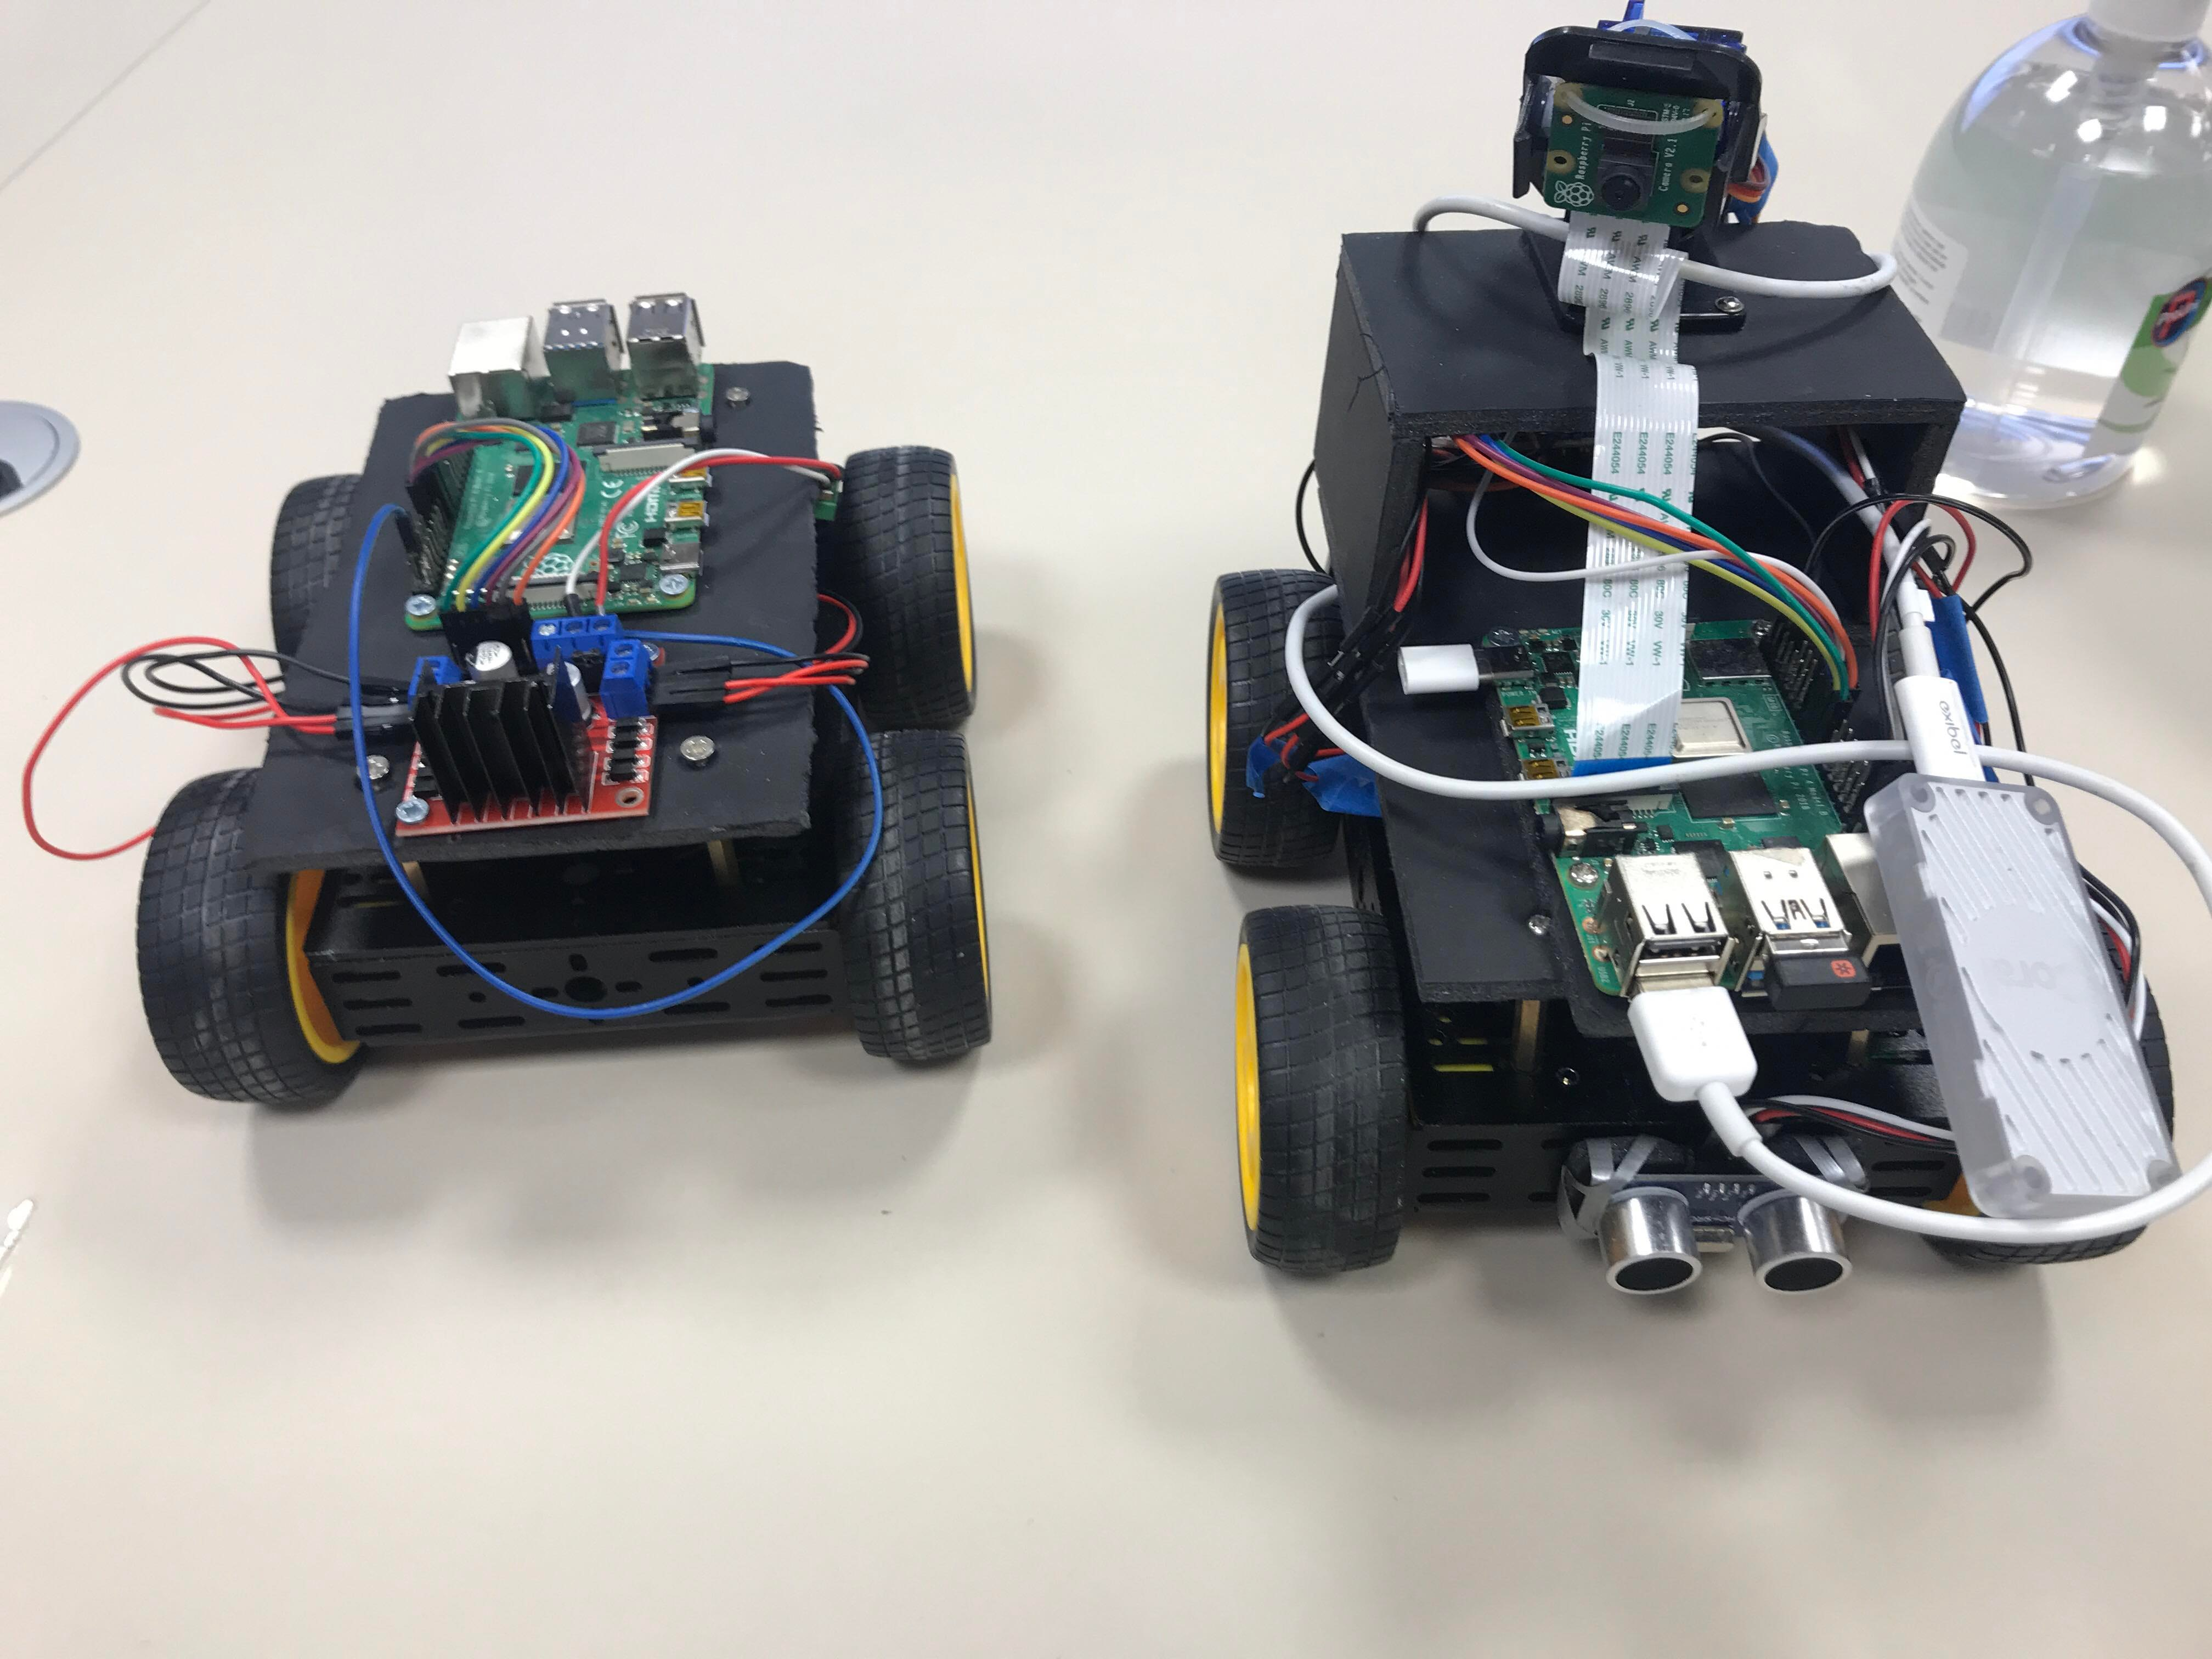
\includegraphics[width=0.9\linewidth]{figures/two_cars}
	\caption{Picture of the two cars we built. To the left is the car without a camera. To the right is the car with a camera on top and a Coral USB Accelerator Edge TPU. This car can take advantage of the onboard AI.}
	\label{fig:twocars}
\end{figure}



